\chapter{随机数的产生}

随机模拟的关键是高质量的随机数。但计算机是一个确定性主导的系统。它无法
产生真正的随机数。因此,我们要么专门构建特殊的装置来产生真随机数,要么
通过一些数学公式来产生性质接近真随机数的伪随机数\cite{Kang2015MonteCarlo}。

\section{真随机数产生器}

真随机数产生器是一种物理装置,它依赖客观世界中的真实随机现象如基本粒子
的随机热运动,量子效应等来产生随机数。这种装置能产生几乎完美的随机数,
但往往产生效率不高,且装置本身较为昂贵。一种可以考虑的方法是使用真随机
数产生器生成的随机数表。比如网站:\\
\href{https://www.random.org}{https://www.random.org} \\
就提供这样的服务。
表\ref{table::random_org}是它的一张价格表。

\begin{table}
  \centering
  \begin{tabular}[!ht]{lll}
    \multicolumn{3}{l}{\bf Integers}\\
    \multicolumn{3}{l}{\bf Prices of Example Files}\\
    \hline
    \hline
Integers & Size of Range  & Price \\
\hline
50,000	& 10	& \$5.00 \\
\hline
250,000	& 1,000	& \$5.00 \\
\hline
1,000,000 & 100	& \$6.66 \\
\hline
5,000,000 & 1,000 & \$36.17 \\
\hline
10,000,000 & 1,000 & \$61.09\\
\hline
\end{tabular}
  \caption{网站 \href{https://www.random.org}{https://www.random.org}
    提供的随机整数表的价格。}
  \label{table::random_org}
\end{table}

随着伪随机数理论和实际质量的提高,以及真随机数在巨型计算系统上的应用限
制,如Monte Carlo法这样随机算法已经没有必要再使用真随机数,高质量的伪
随机数生成算法完全可以胜任。在继续讨论之前,我们先给出随机数的定义。

\begin{definition} {\hei 随机数} 从均匀分布$U(0, 1)$抽样得到的简单子样称为随机数,
  其概率密度函数为
  $$
  f(x) = 1, 0 \leq x \leq 1.
  $$
  随机数用专门符号$U$表示,序列$\{U_1, U_2, \cdots\}$代表独立同分布
  的随机序列。
  \label{def::psudo_random_number}
\end{definition}

随机数的一个非常重要的性质是高维分布均匀性。由$s$个随机数所组成的$s$维
空间上的点
$$
(U_{n + 1}, U_{n + 2}, \cdots, U_{n + s})
$$在$s$维空间的单位正方体$C_s$上是均匀分布的,即$\forall 0 \leq a_i
\leq 1$,$i = 1, 2, \cdots, s$,$U_{n + i} \leq a_i$的概率为:
\begin{equation}
  P(U_{n + i} \leq a_i, i = 1, 2, \cdots, s) = \prod_{i = 1}^s a_i.
\end{equation}

用数学方法产生的随机数称为伪随机数。Tezuka 1995 \cite{Shu1995Uniform}
提出伪随机数应该具有如下特点:
\begin{enumerate}
  \item 能通过统计检验;
  \item 有数学理论支撑;
  \item 可以递推产生,不用占用大量内存;
  \item 产生速度快,效率高;
  \item 重复周期长,至少有$10^{50}$;如果问题需要$N$个随机数,则周期需
    要$2N^2$;
  \item 并行性好,可在计算集群上快速产生;
\end{enumerate}

\section{早期伪随机数算法}

\subsection{经典Fibonacci产生器}

Taussky和Todd 1956年\cite{TausskyGeneration}提出可以用加法同余产生在
$[0, M-1]$均匀分布的伪随机整数,其递推公式为
\begin{equation}
  X_i = (X_{i - 2} + X_{i - 1})\mod M, i > 2.
  \label{eq::add_mod}
\end{equation}
当$X_0 = X_1 = 1$时,公式(\ref{eq::add_mod})产生的序列在小于$M$部分就是
Fibonacci序列,因此又称为经典Fibonacci产生器。该算法过程实现很简单。算
法\ref{alg::add_mod}给出了它的程序。显然,$U_i = X_i / M$给出了相应的
$U(0, 1)$分布随机数。

\begin{minipage}[!ht]{0.8\textwidth}
\vspace{3ex}
\refstepcounter{alg}
\label{alg::add_mod}
\begin{center}
 算法 \arabic{chapter}.\arabic{alg} 加法同余产生器
\end{center}
\small
\begin{tabular}{lll}
  \hei 输入&X0,X1&初值\\
  &M&最大整数值\\
  &N&随机数个数\\
  \hei 输出&&N个服从$U(0, 1)$分布的随机浮点数序列
\end{tabular}
\begin{lstlisting}[style = python]
def rand_add_mod(X0, X1, M, N):
    X = np.zeros(N)
    X[0] = X0
    X[1] = X1
    for i in range(2, N):
        X[i] = (X[i - 2] + X[i - 1]) % M
    return X / (M - 1)
\end{lstlisting}
\end{minipage}

尽管在简单的测试中,这个方案给出的伪随机数似乎还不错,比如图
\ref{fig::add_mod_random_test}中,我们看到在该序列的投点似乎非常均匀。
然而,在特殊的抽样公式
\begin{eqnarray}
  X_i & = & \sqrt{U_i} \cos(2 \pi U_{i + 1}) \sin(\pi U_{i + 2})
  \label{eq::add_mod_random_fail_x}\\
  Y_i & = & \sqrt{U_i} \sin(2 \pi U_{i + 1}) \sin(\pi U_{i + 2})
  \label{eq::add_mod_random_fail_y}
\end{eqnarray}
下,我们看到$X_i$和$Y_i$与应有的统计预测不符。见图
\ref{fig::add_mod_random_fail}。这说明,抽样公式
(\ref{eq::add_mod_random_fail_x})和(\ref{eq::add_mod_random_fail_y})实
际上回归出了加法同余产生器的规律。这在实际模拟中是非常危险的。除此以外,
文献指出,该算法还有其他较为严重的问题,比如随机序列不能居中$(U_i,
U_{i + 1}, U_{i + 2})$在3维空间分布相关等等。但同余运算在伪随机数生成
算法中,仍具有一定的意义。不少现在仍在使用的方法,是经典Fabonacci方法
的一个改进。

\begin{figure}[!ht]
\centering
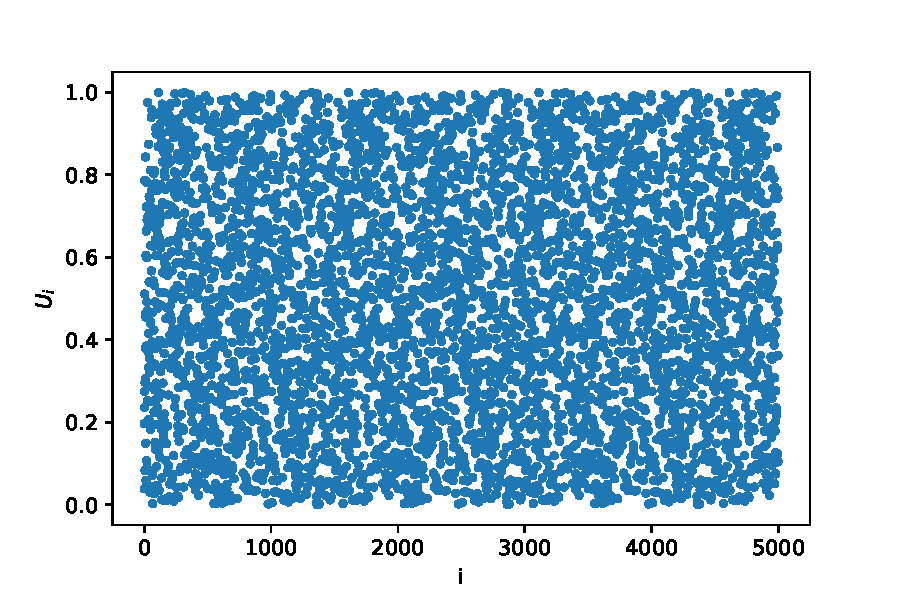
\includegraphics[width=0.7\textwidth]{images/add_mod_random_test.pdf}
\caption{加法同余产生器的均匀性测试, $X_0 = 197$,$X_1 = 39$, $M =
  1000$,一共产生了5000个随机数。}
\label{fig::add_mod_random_test}
\end{figure}

\begin{figure}[!ht]
\centering
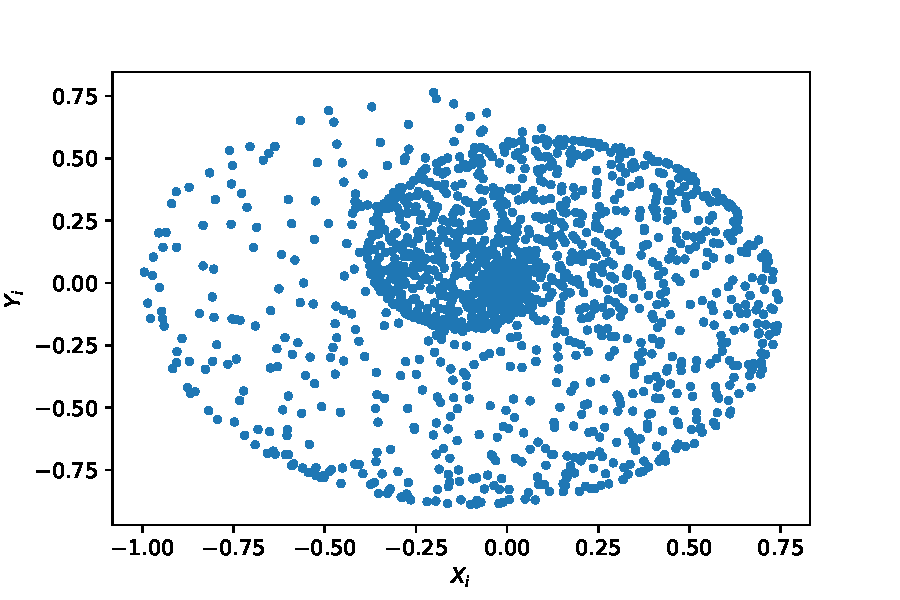
\includegraphics[width=0.7\textwidth]{images/add_mod_random_fail.pdf}
\caption{加法同余产生器的缺陷。在特殊抽样下与统计预测不符。$X_i$和
  $Y_i$分别用公式(\ref{eq::add_mod_random_fail_x})和
  (\ref{eq::add_mod_random_fail_y})产生。}
\label{fig::add_mod_random_fail}
\end{figure}

\subsection{线性同余产生器}

Lehmer 1951\cite{Lehmer1949Mathematical}和Rotenberg
1960\cite{Rotenberg1960A}分别提出了乘同余和混合同余产生器。递推公式为:
\begin{equation}
  X_i = (A * X_{i - 1} + C) \mod M,
  \label{eq::mul_mod}
\end{equation}
其中参数$M$,$A$和$C$分别称为模,乘子和增量。当$C = 0$的特例即是乘同余
产生器,而$C > 0$则称为混合同余产生器。同样可以用$U_i = X_i / M$将其调
整为$U(0, 1)$分布。算法\ref{alg::mul_mod}给出了具体的产生程序。

\begin{minipage}[!ht]{0.8\textwidth}
\vspace{3ex}
\refstepcounter{alg}
\label{alg::mul_mod}
\begin{center}
 算法 \arabic{chapter}.\arabic{alg} 混合同余产生器
\end{center}
\small
\begin{tabular}{lll}
  \hei 输入&X0&初值\\
  &M&最大整数值\\
  &A,C&人工参数\\
  &N&随机数个数\\
  \hei 输出&&N个服从$U(0, 1)$分布的随机浮点数序列
\end{tabular}
\begin{lstlisting}[style = python]
def rand_mul_mod(X0, M, A, C, N):
    X = np.zeros(N)
    X[0] = X0
    for i in range(1, N):
        X[i] = (A * X[i - 1] + C) % M
    return X / (M - 1)
\end{lstlisting}
\end{minipage}

不恰当地选择参数也会有有类似加同余的异常相关现象,
图\ref{fig::mul_mod_random_fail} 对参数$A = 7$,$M = 2^{31} - 1$给出在
特殊抽样
\begin{eqnarray}
  X_i & = & \sqrt{-2 \ln U_i} \cos(2 \pi U_{i + 1}) 
  \label{eq::mul_mod_random_fail_x}\\
  Y_i & = & \sqrt{-2 \ln U_i} \sin(2 \pi U_{i + 1}) 
  \label{eq::mul_mod_random_fail_y}
\end{eqnarray}
下的二维分布图。可以看到样本点全部落在一条螺旋线上。

\begin{figure}[!ht]
\centering
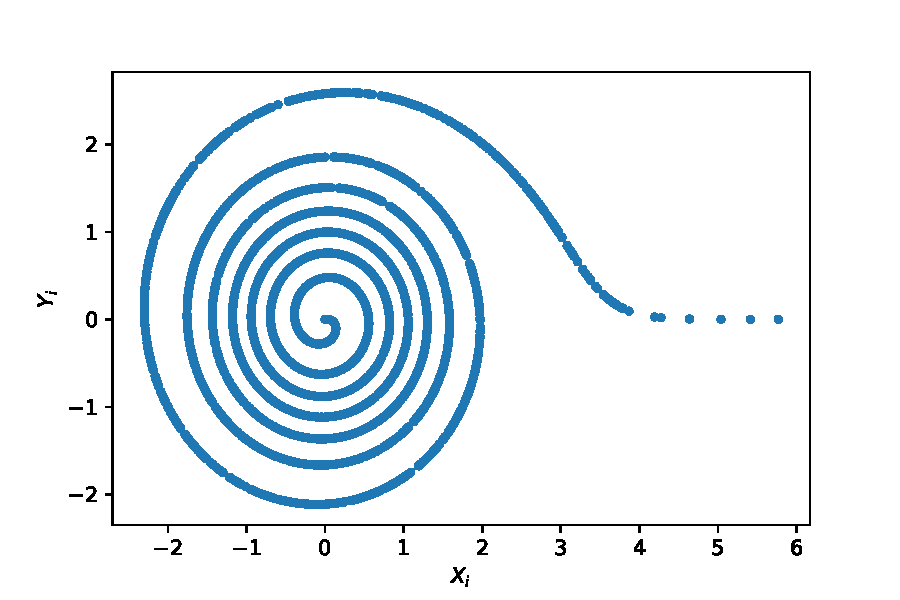
\includegraphics[width=0.7\textwidth]{images/mul_mod_random_fail.pdf}
\caption{线性同余产生器的缺陷。$X_i$和$Y_i$分别用公式
  (\ref{eq::mul_mod_random_fail_x})和(\ref{eq::mul_mod_random_fail_y})
  产生。所有的点都落在一条螺旋线上。}
\label{fig::mul_mod_random_fail}
\end{figure}

线性同余产生器的参数选择需要一些数论的概念。首先引入定义:

\begin{definition} {\hei 原根(Primitive Root)}
  称线性同余产生器参数乘子$A$是模$M$的原根,当且仅当
  \begin{enumerate}
    \item 
      \begin{equation}
        (A^{M - 1} - 1) \mod M  = 0;
        \label{eq::primitive_root}
      \end{equation}
    \item 任取$I < M - 1$, $(A^I - 1) / M$不是整数.
  \end{enumerate}
  \label{def::primitive_root}
\end{definition}

我们总是希望伪随机数的周期尽可能长(伪随机数周期总是会有的),在
\cite{Fishman1995Monte}中,作者指出当模$M$是素数时,当且仅当乘子$A$是
其原根时,乘同余产生器的周期是$M - 1$。因此我们一般将$M$取成$2^\beta -
1$(梅森数),这里$\beta$是机器字长。而对于混合同余产生器,模$M$一般取
$2^\beta$,其周期为$M$当且进当$A = 4k + 1$,$k \in \mathbb{N}$,且$M$
和$C$互质。

线性同余方法曾经广泛使用于各个计算机平台做为伪随机数发生器。比如IBM
360系统下曾有一个著名的随机数产生器RANDU被使用多年。它就是$A = 65539$,
$M = 2^{31}$的线性乘同余产生器。然而,可以验证,它的三重分布,即
$(U_{i}, U_{i + 1}, U_{i + 2})$只分布在15个空间平面上见图
\ref{fig::RANDU_fail},它们是:
\begin{equation}
  9x - 6y + z = k, k = -5, -4, \cdots, 8, 9.
\label{eq::RANDU_plain}  
\end{equation}
这一现象被称为降维,它导致随机数的高维分布均匀性消失。具体推导可参见:\\
\href{https://en.wikipedia.org/wiki/RANDU}{https://en.wikipedia.org/wiki/RANDU} \\

\begin{figure}[!ht]
\centering
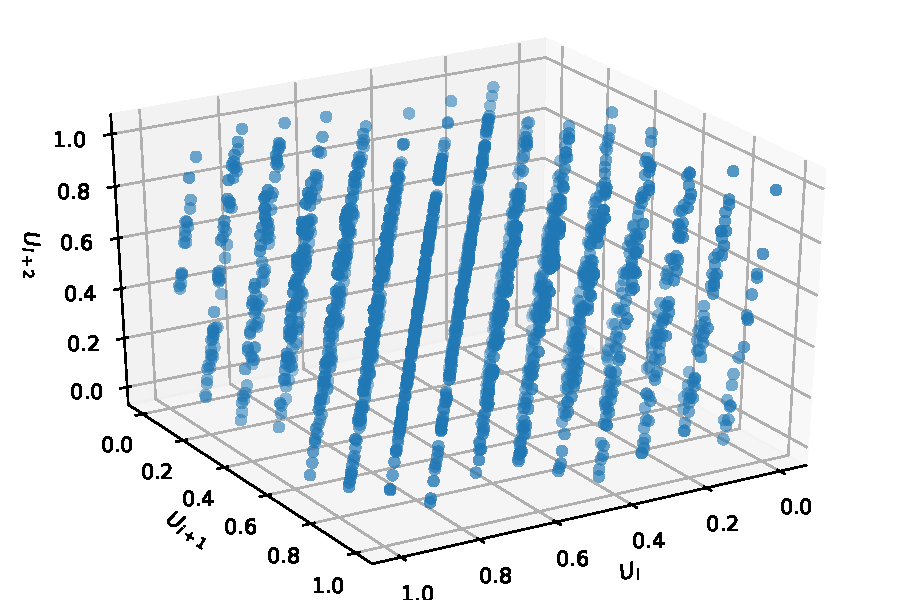
\includegraphics[width=0.7\textwidth]{images/RANDU_fail.pdf}
\caption{IBM360/370 RANDU的三维分布稀疏栅格现象。这里$A = 65539$,$M =
  2^{31}$,$C = 0$。}
\label{fig::RANDU_fail}
\end{figure}

可以证明,降维现象是线性同余产生器的一个必然结果。一般地,对与线性同余
产生器产生的伪随机点列构成的$s$维空间点列
\begin{equation}
  P = (U_i, U_{i + 1}, \cdots, U_{i + s - 1}), i = 1, 2, \cdots
  \label{eq::mul_mod_mul_dim_fail}
\end{equation}
只落在个数不超过$(s!M)^{1/s}$的彼此平行的超平面上(参见:
  \cite{Marsaglia1968Random})。

由于以上这些缺陷,目前的主流意见是不要单独使用线性同余产生器。特别是在
进行类似Monte Carlo模拟时,要格外警惕伪随机数的降维和异常相关现象。当
我们在具体的系统上运算时,也应该先阅读文档,查找具体的随机数产生方式。
比如,某些低版本的GCC编译器提供的伪随机数就有可能是$M = 2^{32}$,$A =
1103515245$,$C = 12345$的一个混合同余产生器。

\section{伪随机数产生器的进展}

线性同余算法尽管快速简单,但由于它的缺陷,人们陆续提出了一些新的算法以
产生更高质量的随机数。主要的改进思路来自以下几个方向:

\subsection{非线性同余产生器}
这种生成器的思想是当$M$是素数时,通过构建某种排列多项式,将$\{0, 1,
\cdots, M -1\}$作为一个Galois域重排成$\{g(0), g(1), \cdots, g(M -
1)\}$,然后在此基础上构建递推生成器。以继承这种基于重排的均匀性。

比如逆同余产生器:
\begin{equation}
  X_i = (A X_{i - 1}^{-1} + C) \mod M, i \geq 1.
  \label{eq::inv_lin}
\end{equation}
这里的$g(x) = x^{-1}$是一种非线性整函数,定义为:

\begin{definition} {\hei 乘法逆(multiplicative inverse)}
  称$z^{-1}$是$z$关于$M$的乘法逆,如果
  \begin{equation}
    z \cdot z^{-1} \mod M = 1, z^{-1} \in \mathbb{N}, z^{-1} < M.
    \label{eq::mul_inv}
  \end{equation}
  \label{def::mul_inv}
\end{definition}
并且规定$0$的乘法逆为$0$。

可以验证,对$M = 11$,$A = 8$,$C = 1$和$X_0 = 0$产生的前9个数是
$$
0, 1, 9, 8, 2, 5, 7, 10, 4, 3,
$$基本上就是$0 \sim 10$的重排(漏掉了6以外)。这种产生器可以通过很高维
的栅格检验,但是它的生成效率远低于线性同余。关于如何高效求乘法逆涉及数
论、群论和计算机算法的高深内容,有兴趣的同学可参见
\cite{Lidl1986Introduction}.

此外,常用的非线性同余产生器还有二次或高次同余,二次同余递推公式为:
\begin{equation}
  X_i = (A X_{i - 1}^2 + B X_{i - 1} + C) \mod M.
  \label{eq::q_mod}
\end{equation}
更多的内容可自行参考\cite{Fishman1995Monte, Kang2015MonteCarlo}。

\subsection{多步线性递推产生器}
即增加线性递推的递推层数,一般性的多步线性递推公式为:
\begin{equation}
  X_i = (A_1 X_{i - 1} + A_2 X_{i - 2} + \cdots + A_j X_{i - j}) \mod
  M, i \geq j.
  \label{eq::mul_lin}
\end{equation}
为提高效率,一般我们只保留其中两个系数$A_j$和$A_l$不为零,由此产生了一
系列具体的方案:

\begin{enumerate}
\item FMRG($A_1 = 1$,$A_l = B$),
  \begin{equation}
    X_i = (X_{i - 1} + B X_{i - l}) \mod M;
    \label{eq::fmrg}
  \end{equation}
\item DX-k-2($A_1 = A_l = B$),
  \begin{equation}
    X_i = B(X_{i - 1} + X_{i - l}) \mod M;
    \label{eq::dxk2}
  \end{equation}
\item DX-k-3($A_1 = A_{[l / 2]} = A_l = B$),
  \begin{equation}
    X_i = B(X_{i - 1} + X_{i -[1 / 2]} + X_{i - l}) \mod M;
    \label{eq::dxk3}
  \end{equation}
\item DX-k-4($A_1 = A_{l / 3} = A_{[2l /3]} = A_l = B$),
  \begin{equation}
    X_i = B(X_{i - [l /3]} + X_{i - [2l /3]} + X_{i - l}) \mod M.
  \end{equation}
\end{enumerate}
以上,$i \geq l$。这一系列公式的极致是L. Y. Deng 等人2003年设计的
DX3803生成器,周期长达$2^{117923}$,而且在3803维空间内分布均匀。参见:
\cite{Deng2003A}。

除了上面的方案,常用的改良手段还有进位借位运算产生器\cite{Shu1993On},
延迟Fibonacci生成器\cite{Brent1992Uniform},线性同余组合产生器
\cite{L1991Structural, Rose2014KISS},混合组合产生器
\cite{Fischer1999Good, Marsaglia2004The, Marsaglia1990Toward}等等,限
于篇幅不一一叙述,有兴趣的同学请自行查阅文献。

\section{梅森旋转(Mersenne Twister)产生器}

最后我们介绍一种目前最广泛使用的随机数产生器——梅森旋转产生器。它基于四
位日本数学家所发表的一系列论文,Matsumoto(松本) \& Kurita(栗田)
1992, 1994\cite{Matsumoto1992Twisted, Matsumoto1994Twisted},Matsumoto
\& Nishimura(西村) 1998, 2000
\cite{Matsumoto2000Dynamic, Matsumoto1998Mersenne},Matsumoto \& Saito(斋藤)
2008\cite{Saito2008SIMD}。它的一个重要实例MT19937被几乎所有重要编程平
台包括并不限于:C,C++,Python,Matlab等所采纳。它周期长达$2^{19937}-1$,
能通过目前几乎所有的随机数检验程序,且在至多623维空间分布均匀。MT19937
是基于32位字长机器运算。下面我们来介绍MT19937的具体实现过程。本章代码在
cnblog上网友xlxw的blog《Python下探究随机数的产生原理和算法》,网址:\\
\href{https://www.cnblogs.com/lzxwalex/p/6880748.html}
     {https://www.cnblogs.com/lzxwalex/p/6880748.html} \\
提供的代码基础上修改而成,并参考了CSDN网友tick\_tokc97的blog
《伪随机数生成——梅森旋转(Mersenne Twister/MT)算法笔记》\\
\href{https://blog.csdn.net/tick_tock97/article/details/78657851}
     {https://blog.csdn.net/tick\_tock97/article/details/78657851}。


\subsection{初始化}
梅森旋转需要有一个工作区。MT19937的工作区是一个长度为624的数组,每个元
素都是32位字长的整数。生成工作区的过程称为初始化。初始化本身也是一个伪
随机数产生过程,这个过程采用了类似线性产生器,并混合了位运算以保证产生
数字在二进制位的形式上分布均匀。具体公式为:
\begin{equation}
  M_i = f * (M_{i - 1} \oplus (M_{i - 1} >> (w - 2))) + i, i = 1, 2, \cdots, 624.
  \label{eq::MT19937_init}
\end{equation}
这里32位整数向量$M$存放的就是工作区,$M_0$由用户作为种子给出,$f$是
参数,在MT19937中取1812433253(十六进制:6C078965)。运算符$\oplus$表
示异或运算XOR,$w$表示机器字长,在MT19937中取32。具体的算法代码见算法
\ref{alg::MT19937_init},

\begin{minipage}[!ht]{0.8\textwidth}
\vspace{3ex}
\refstepcounter{alg}
\label{alg::MT19937_init}
\begin{center}
 算法 \arabic{chapter}.\arabic{alg} MT19937工作区初始化
\end{center}
\small
\begin{tabular}{lll}
  \hei 输入&seed&随机数种子\\
  &M&存储梅森工作区的空间\\
  \hei 输出&&生成的梅森工作区
\end{tabular}
\begin{lstlisting}[style = python, escapechar = \%]
# 转换成32位整数。
def inter(t):
    return(0xFFFFFFFF & t) #截取最后32位

def mainset(seed, M):
    M[0] = seed    
    for i in range(1,624):
        M[i] = inter(1812433253 * (M[i - 1] ^ M[i - 1] >> 30) + i)
    return M
\end{lstlisting}
\end{minipage}

初始化本身就是一个还算不错的伪随机数产生器。

\subsection{梅森旋转}
接下去通过梅森旋转,直接从二进制层面在整个工作区重新分布0和1,并且用旋
转和异或操作使二进制数分布均匀。由于工作区的长度是624,故每产生624个数,
都要重新执行一次梅森旋转。
\begin{equation}
  M_i = M_{i + m} \oplus ((\mbox{upper\_mask}(M_i) ||
  \mbox{lower\_mask}(M_{i+1}))A)
  \label{eq::MT19937_twister}
\end{equation}
此处,$\mbox{upper\_mask}(M_i)$和$\mbox{lower\_mask}(M_{i + 1})$分别表
示取$M_i$和$M_{i + 1}$的高$w - r$位和低$r$(在MT19937中$w = 32$,$r =
  31$),符号$||$表示将两边的高位和低位连接成一个32位的数。下一步$xA$
运算的定义为:
\begin{equation}
  xA = \left\{
  \begin{array}{ll}
    x >> 1, & x_0 = 0, \\
    (x >> 1) \oplus a, & x_0 = 1.
  \end{array}
  \right.
\end{equation}
这里$x_0$表示$x$的最低位,$a$是给定参数,在MT19937中设置为
0x9908B0DF(十六进制)。最后将$i$后第$m$个工作区数(在MT19937中$m =
  397$),即$M_{i + m}$拿来和连接成的数做异或,注意上述下标$i + 1$和$i
+ m$在实际实现中都要和624取模,因此实际上整个工作区是循环边界的。这也
是梅森旋转的名字中旋转的来历。完整的算法过程见算法
\ref{alg::MT19937_twister}。

\begin{minipage}[!ht]{0.8\textwidth}
\vspace{3ex}
\refstepcounter{alg}
\label{alg::MT19937_twister}
\begin{center}
 算法 \arabic{chapter}.\arabic{alg} MT19937梅森旋转
\end{center}
\small
\begin{tabular}{lll}
  \hei 输入&梅森工作区的空间\\
  \hei 输出&旋转后的梅森工作区
\end{tabular}
\begin{lstlisting}[style = python]
def twister(M):
    for i in range(624):
        # 截取M[i]高位和M[i+1](越界就返回M[0])低位,用普通加法合并,对齐32位
        # 这里高位取了1位,低位取了31位。
        y = inter((M[i] & 0x80000000) +(M[(i + 1) % 624] & 0x7fffffff))
        yA = y >> 1
        if y & 1 == 1: #取最低位
            yA = yA ^ 0x9908b0df
        M[i] = M[(i + 397) % 624] ^ yA
    return M
\end{lstlisting}
\end{minipage}

\subsection{递推}
最后我们可以利用工作区,产生梅森旋转的递推公式:
\begin{eqnarray}
  y &=& x \oplus ((x >> u) \& d),\\
  \label{eq::MT19937_recursion1}
  y &=& y \oplus ((y << s) \& b),\\
  \label{eq::MT19937_recursion2}
  y &=& y \oplus ((y << t) \& c), \\
  \label{eq::MT19937_recursion3}
  z &=& y \oplus (y >> l). 
  \label{eq::MT19937_recursion4}
\end{eqnarray}
这里$x$依次从$M$中取,取完624个则重新执行梅森旋转。$y$是中间变量,$z$
是返回的下一个随机数。其他$u$,$d$,$s$,$b$,$t$,$c$和$l$均为人工参数。在
MT19937中,$l = 18$,其余参数分别取作
\begin{eqnarray*}
  (u, d) &=& (11, \mbox{0xFFFFFFFF$_{16}$}),\\
  (s, b) &=& (7, \mbox{0x9D2C5680$_{16}$}),\\
  (t, c) &=& (15, \mbox{0xEFC60000$_{16}$}), \\
\end{eqnarray*}
这里第二列都是十六进制。

最后,完整的随机数生成算法见\ref{alg::MT19937}。

\begin{minipage}[!ht]{0.8\textwidth}
\vspace{3ex}
\refstepcounter{alg}
\label{alg::MT19937}
\begin{center}
 算法 \arabic{chapter}.\arabic{alg} MT19937主流程
\end{center}
\small
\begin{tabular}{lll}
  \hei 输入&seed&随机数种子\\
  &num&随机数个数\\
  \hei 输出&&num个服从$U(0, 1)$分布的随机浮点数序列
\end{tabular}
\begin{lstlisting}[style = python]
def exnum(M, index):
    y = M[index]
    y = y ^ y >> 11
    y = y ^ y << 7 & 2636928640
    y = y ^ y << 15 & 4022730752
    y = y ^ y >> 18
    index = index + 1
    return inter(y)
    
def MT19937(seed, num):
    U = [0]*num
    M = [0]*624
    M = mainset(seed, M)
    twister(M)
    for i in range(num):
        index = i % 624
        U[i] = exnum(M, index) / (2**32 - 1)
        if (index == 623):
            twister(M)
    return U     
\end{lstlisting}
\end{minipage}

由于梅森旋转当中大量核心算法是位运算,因此运算效率极高,且便于机器底层
实现。这也是它成为目前最通用和最受欢迎的伪随机数生成算法。它同样也有64
和128位版本。其作者还在不断提高其计算效率和随机数质量,最新的进展可参
见广岛大学提供的网站:\\
\href{http://www.math.sci.hiroshima-u.ac.jp/~m-mat/MT/emt.html}
     {http://www.math.sci.hiroshima-u.ac.jp/~m-mat/MT/emt.html}。

\section{多维随机数产生方法}
多维随机数有直接产生的方法,具体参见Niederreiter
1992\cite{Niederreiter1992Random},这种方法产生的多维随机数性质较好,
但更为简便的方法是基于下述概率论定理用一维随机数间接产生:

\begin{theorem}
  若$\{A_i, i = 1, 2, \cdots, ns\}$是独立同分布的随机变量序列,
  则
  \begin{equation}
    \{(A_{(i - 1)s + 1}, A_{(i - 1)s + 2}, \cdots, A_{is}), i = 1, 2, \cdots\}
    \label{thm::mulvar}
  \end{equation}
  必是$s$维独立同分布的随机向量序列。而且每个分量序列
  \begin{equation}
    \begin{array}{rcl}
      \mathrm{U}_1 &=& \{U_1, U_{s + 1}, \cdots, U_{(n - 1)s + 1}\},\\
      \mathrm{U}_2 &=& \{U_2, U_{s + 2}, \cdots, U_{(n - 1)s + 2}\},\\
      &\cdots&\\
      \mathrm{U}_s &=& \{U_s, U_{2s}, \cdots, U_{ns}\},
    \end{array}
  \end{equation}
  在各自的维度中也是独立同分布的。
\end{theorem}

我们用上面的MT19937产生一维50万个随机数,并按定理次序重新组织成500个
1000维的随机向量。观察一下$(U_1, U_2)$和$(U_{999}, U_{1000})$平面的随
机数分布,都很均匀(见图\ref{fig::MT19937_1000D})。

\begin{figure}[!ht]
\centering
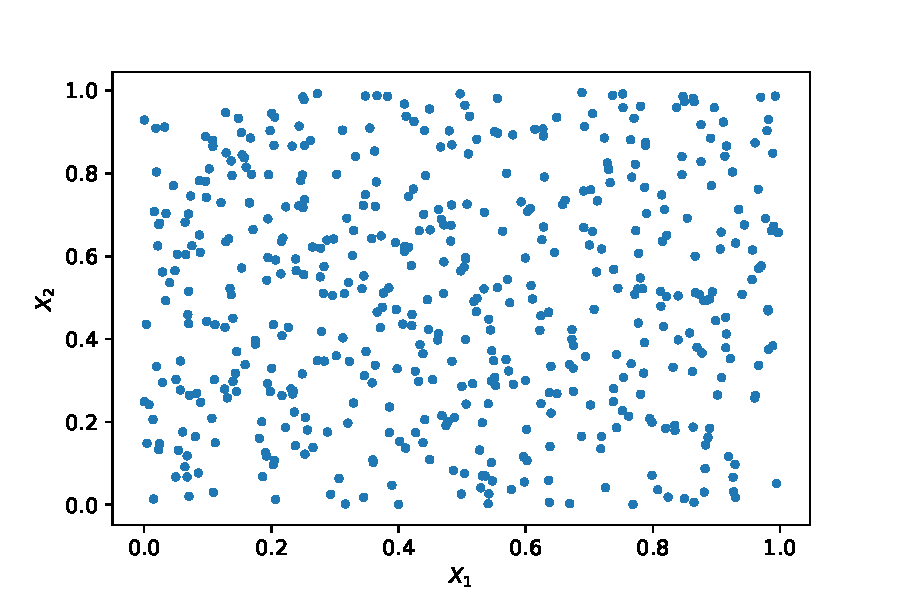
\includegraphics[width=0.45\textwidth]{images/MT19937_X1X2.pdf}
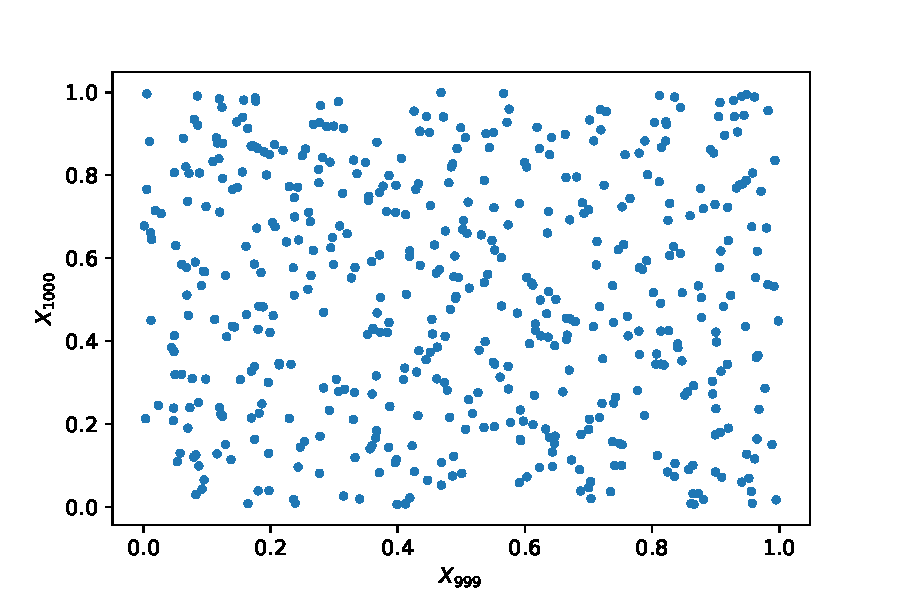
\includegraphics[width=0.45\textwidth]{images/MT19937_X999X1000.pdf}
\caption{用MT19937生成50万个随机数,重新组织成500个1000维随机向量。左
  图和右图分别是第$(1, 2)$维和第$(999, 1000)$维平面的随机数分布情况。}
\label{fig::MT19937_1000D}
\end{figure}

\section{随机数的检测}

随机数的理论检测即从随机数的产生原理出发,寻找它的缺陷。比如之前的栅格
现象(图\ref{fig::RANDU_fail})等。实际上这种缺陷也是在应用过程中发现,
才被人们所重视,并且在设计随机数产生器时格外注意。理论检验都只针对具体
的产生原理,并没有一般性。更多的,我们需要用现代统计学手段对随机数的质
量进行统计分析。较为一般的检验,可以是检查随机数的频率,频次,相关性,
各阶矩等等。更复杂的检验,则要精确设计统计实验,并涉及到较为复杂和专业
的统计学知识。目前被大家所接受的统计学检验程序是Marsaglia给出的DieHard
程序。它由一系列精心设计的复杂统计实验组成,几乎是目前检测随机数质量的
标准过程。George Marsaglia教授已于2011年去世,但DieHard程序仍然有人不
断更新和维护,并引入了GPL协议使得可以公开下载和免费使用。具体可参见网
站:\\
\href{http://webhome.phy.duke.edu/\~rgb/General/dieharder.php}
     {http://webhome.phy.duke.edu/~rgb/General/dieharder.php}
     \\

     
